\begin{comment}



\begin{frame}{Redondances intra-règle}
     Deux formes de redondances statiques étudiées :

    \begin{itemize}
    \color{red}
        \item Les redondances intra-règle 
        \color{black}
        \item Les redondances inter-règle 
       
    \end{itemize}
\end{frame}{}

\end{comment}

\begin{frame}{Redondances intra-règle}

    Il existe 2 formes de redondances intra-règle :

    \begin{itemize}
        \item Les redondances du corps dans le corps de la règle ; 
        \item Les redondances de la tête sur le corps et la tête de la règle
    \end{itemize}
    
    On va présenter la deuxième forme de redondance.
   
\end{frame}


%
%\begin{frame}[fragile]{Redondances intra-règle}
%    Les redondances du corps dans le corps de la règle :
    
%    \begin{block}{Exemple}
%        Soit la règle $R = p(X) \land p(Y) \xrightarrow{} q(X,Z)$.
%    \end{block}
    
%    Si $R$ est appliquée on aura la base de faits $\mathcal{F} = \{p(X),  p(Y), q(X,Z_1)\}$.
    
 %     \begin{block}{Le graphe représentant $\{p(X),  p(Y), q(X,Z_1)\}$}
 %    \begin{tikzpicture}[->,>=stealth,shorten >=1pt,auto,node distance=2.5cm,
%                thick,main node/.style={circle,draw,font=\Large\bfseries,scale=0.6}]
%    \node[main node] (1) {$X$};
%  \node[main node] (2) [below of=1] {$Y$};
%  \node[main node] (3) [right of=2] {$Z_1$};

%  \path
%    (1) edge [loop above] node {p} (1)
%    (1) edge (3)
%    (2) edge [loop above] node {p} (2)
%  ;
%\end{tikzpicture}
%\end{block} 
%\end{frame}


%\begin{frame}{Redondances intra-règle}
    
%    Les redondances du corps dans le corps de la règle :
    
%    \begin{block}{Exemple}
%        Soit la règle $R = p(X) \land p(Y) \xrightarrow{} q(X,Z)$.
%    \end{block}
    
%    Si on calcul le \textit{core} à la base de faits $\mathcal{F}$ on obtient $\mathcal{F}'  = \{p(X), q(X,Z_1)\}$.
    
%     \begin{block}{Le graphe représentant $\{p(X),  q(X,Z_1)\}$}
%     \begin{tikzpicture}[->,>=stealth,shorten >=1pt,auto,node distance=2.5cm,
 %               thick,main node/.style={circle,draw,font=\Large\bfseries,scale=0.6}]
 %   \node[main node] (1) {$X$};
 % \node[main node] (3) [right of=2] {$Z_1$};

  %\path
  %  (1) edge [loop above] node {p} (1)
  %  (1) edge (3)
 % ;
%\end{tikzpicture}
%\end{block} 
    
%\end{frame}
    

\begin{frame}{Redondances intra-règle}

    
    \begin{block}{Les redondances de la tête sur le corps et la tête de la règle }
    On va chercher les atomes redondant et les supprimer tout en maintenant le corps car on cherche les redondances de la tête sur corps.
    \end{block}
\end{frame}

\begin{frame}{Redondances intra-règle}
   
    \begin{block}{Comment supprimer ces redondances ? }
        On va calculer le \textit{core} de l'union des atomes du corps dont les variables sont gelés et les atomes de la tête de la règle. 
    \end{block}
    
  
    
\end{frame}

\begin{frame}{Redondances intra-règle}

    Les redondances de la tête sur le corps et la tête de la règle :
    \begin{block}{Exemple}
        Soit la règle $R = p(X,Y) \xrightarrow{} p(Y,Z) \land p(T,Z) \land p(S,T)$.
    \end{block}
    Si on applique le \textit{core} à la base de faits $\mathcal{F}$, on obtient $\mathcal{F}' = \{p(X_f,Y_f),  p(Y_f,Z)\}$.
       \begin{block}{Le graphe représentant $\{p(X_f,Y_f),  p(Y_f,Z), p(T,Z) , p(S,T)\}$}
 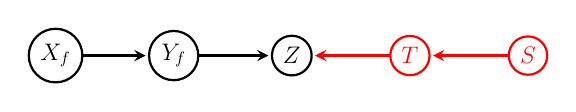
\begin{tikzpicture}[->,>=stealth,shorten >=1pt,auto,node distance=2.5cm,
                thick,main node/.style={circle,draw,font=\Large\bfseries,scale=0.6}]
  \node[main node] (1) {$X_f$};
  \node[main node] (2) [right of=1] {$Y_f$};
  \node[main node] (3) [right of=2] {$Z$};
  \node[main node] (4) [right of=3, red] {$T$};
  \node[main node] (5) [right of=4, red] {$S$};

  \path
    (1) edge (2)
    (2) edge (3)
    (4) edge [red] (3)
    (5) edge [red] (4)
  ;
\end{tikzpicture}
\end{block} 
    
    \begin{block}{Le graphe représentant $\{p(X,Y),  p(Y,Z)\}$}
 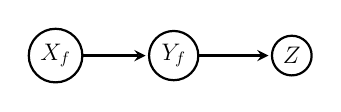
\begin{tikzpicture}[->,>=stealth,shorten >=1pt,auto,node distance=2.5cm,
                thick,main node/.style={circle,draw,font=\Large\bfseries,scale=0.6}]
  \node[main node] (1) {$X_f$};
  \node[main node] (2) [right of=1] {$Y_f$};
  \node[main node] (3) [right of=2] {$Z$};

  \path
    (1) edge (2)
    (2) edge (3)
  ;
\end{tikzpicture}
\end{block} 
\end{frame}

%\begin{frame}{Redondances intra-règles}

  %  Algorithmes pour supprimer les redondances intra-règles :
    
%   \begin{itemize}
 %       \item On calcul le \textit{core} sur le corps de la règle en gelant la frontière
 %       \item On calcul le \textit{core} sur le nouveau corps gelé et la tête de la règle
 %       \item Si la tête est vide on supprime la règle de la base de règles
 %   \end{itemize}
   
%\end{frame}

%\begin{frame}{Redondances intra-règles}

 %   Algorithmes pour supprimer les redondances intra-règles :
    
 %   \begin{itemize}
 %       \item On calcul le \textit{core} sur le corps de la règle en gelant la frontière
 %       \item On calcul le \textit{core} sur le nouveau corps gelé et la tête de la règle
  %      \item Si la tête est vide on supprime la règle de la base de règles
  %  \end{itemize}
    
  %  \begin{block}{Exemple}
  %      Soit la règle $R =  p(X,Y) \land p(X,U) \xrightarrow{} p(Y,Z) \land p(T,Z) \land p(S,T)$
%    \end{block}
   
%\end{frame}

%\begin{frame}{Redondances intra-règles}

 %   Algorithmes pour supprimer les redondances intra-règles :
    
 %   \begin{itemize}
 %       \color{red}
 %       \item On calcul le \textit{core} sur le corps de la règle en gelant la frontière
 %       \color{black}
 %       \item On calcul le \textit{core} sur le nouveau corps gelé et la tête de la règle
 %       \item Si la tête est vide on supprime la règle de la base de règles
 %   \end{itemize}
    
 %   \begin{block}{Exemple}
%        Soit la règle $R =  p(X,Y) \land p(X,U) \xrightarrow{} p(Y,Z) \land p(T,Z) \land p(S,T)$
 %       On gèle la frontière de $R$, ici : $Y$.
 %       Puis on calcul le \textit{core} sur le corps : $\{p(X,Y), p(X,U)\}$ pour obtenir : $\{p(X,Y)\}$. 
 %%        \begin{tikzpicture}[->,>=stealth,shorten >=1pt,auto,node distance=2.5cm,
  %              thick,main node/.style={circle,draw,font=\Large\bfseries,scale=0.6}]
 % \node[main node] (1) {$X$};
 % \node[main node] (2) [right of=1] {$Y$};
%  \node[main node] (3) [left of=1] {$U$};

 %% \path
 %   (1) edge (2)
 % ;
 % \end{tikzpicture}
 
 %   Dont le \textit{core} est : 
 %   \begin{tikzpicture}[->,>=stealth,shorten >=1pt,auto,node distance=2.5cm,
%                thick,main node/.style={circle,draw,font=\Large\bfseries,scale=0.6}]
%  \node[main node] (1) {$X$};
%  \node[main node] (2) [right of=1] {$Y$};

 % \path
 %   (1) edge (2)
 % ;
%  \end{tikzpicture}
%    \end{block}
   
%\end{frame}

%\begin{frame}{Redondances intra-règles}

  %  Algorithmes pour supprimer les redondances intra-règles :
    
  %  \begin{itemize}
%        \item On calcul le \textit{core} sur le corps de la règle en gelant la frontière
 %       \color{red}
  %      \item On calcul le \textit{core} sur le nouveau corps gelé et la tête de la règle
  %      \color{black}
  %      \item Si la tête est vide on supprime la règle de la base de règles
 %   \end{itemize}
    
 %   \begin{block}{Exemple}
 %       Soit la règle $R' =  p(X,Y) \xrightarrow{} p(Y,Z) \land p(T,Z) \land p(S,T)$
 %       On gèle la frontière de $R'$, ici : $Y$.
 %       Puis on calcul le \textit{core} sur le corps et la tête : $\{p(X,Y)\} \bigcup \{p(Y,Z), p(T,Z), p(S,T)\}$. 
 %        \begin{tikzpicture}[->,>=stealth,shorten >=1pt,auto,node distance=2.5cm,
 %               thick,main node/.style={circle,draw,font=\Large\bfseries,scale=0.6}]
 %  \node[main node] (1) {$X$};
  %\node[main node] (2) [right of=1] {$Y$};
%  \node[main node] (3) [right of=2] {$Z$};
%  \node[main node] (4) [right of=3] {$T$};
%  \node[main node] (5) [right of=4] {$S$};

%  \path
%    (1) edge (2)
%    (2) edge (3)
%    (4) edge (3)
%    (5) edge (4)
%  ;
%  \end{tikzpicture}
 
 %   Dont le \textit{core} est : 
 %   \begin{tikzpicture}[->,>=stealth,shorten >=1pt,auto,node distance=2.5cm,
 %               thick,main node/.style={circle,draw,font=\Large\bfseries,scale=0.6}]
%  \node[main node] (1) {$X$};
%  \node[main node] (2) [right of=1] {$Y$};
%  \node[main node] (3) [right of=2] {$Z$};

%  \path
%    (1) edge (2)
%    (2) edge (3)
%  ;
%  \end{tikzpicture}
%    \end{block}
   
%\end{frame}

%\begin{frame}{Redondances intra-règles}

%    Algorithmes pour supprimer les redondances intra-règles :
    
 %   \begin{itemize}
%        \item On calcul le \textit{core} sur le corps de la règle en gelant la frontière
%        
%  \item On calcul le \textit{core} sur le nouveau corps gelé et la tête de la règle
%        \color{red}
%        \item Si la tête est vide on supprime la règle de la base de règles
%        \color{black}
%    \end{itemize}
    
    
 %   \begin{block}{Exemple}
 %       Soit la règle $R =  p(X,Y) \xrightarrow{} p(X,Z)$
 %       On gèle la frontière de $R$, ici : $X$.
 %       Puis on calcul le \textit{core} sur le corps et la tête : 
 %        \begin{tikzpicture}[->,>=stealth,shorten >=1pt,auto,node distance=2.5cm,
  %              thick,main node/.style={circle,draw,font=\Large\bfseries,scale=0.6}]
%   \node[main node] (1) {$X$};
%  \node[main node] (2) [right of=1] {$Y$};
%  \node[main node] (3) [below of=2] {$Z$};

 % \path
 %   (1) edge (2)
 %   (1) edge (3)
%  ;
 % \end{tikzpicture}
 
 %   Dont le \textit{core} est : 
%    \begin{tikzpicture}[->,>=stealth,shorten >=1pt,auto,node distance=2.5cm,
 %               thick,main node/.style={circle,draw,font=\Large\bfseries,scale=0.6}]
 % \node[main node] (1) {$X$};
 % \node[main node] (2) [right of=1] {$Y$};

%  \path
%    (1) edge (2)
%  ;
  
 
%  \end{tikzpicture}
%  On obtient $R' = p(X,Y) \xrightarrow{}$ sans redondances mais qui ne produit plus rien.
%    \end{block}
   
%\end{frame}